\documentclass [a4paper,11pt]{article}
\usepackage{booktabs}
\usepackage{zhfontcfg}
\usepackage{multirow}
\usepackage[margin=1in]{geometry}


\title{用例文档}
\date{\today}
\author{LetsGo安卓应用开发小组}

\begin{document}
	
\maketitle
\section*{修订历史}

\begin{table}[!hbp]
\centering

\begin{tabular*}{\textwidth}{c|c|c|c}
\hline
\rule{0pt}{0.8cm}
版~本 & 日~期 & 描~述 & 作~者\\
\hline
\rule{0pt}{0.6cm}
初始草案 & 2014年6月1日 & 第一个草案。描述最简单但是最重要的用例。 & 陆正毅\\
\hline
\rule{0pt}{0.6cm}
 &  &  & \\
\hline
\end{tabular*}

\end{table}


\section*{部署图}

\begin{figure}[ht!]
			\centering
			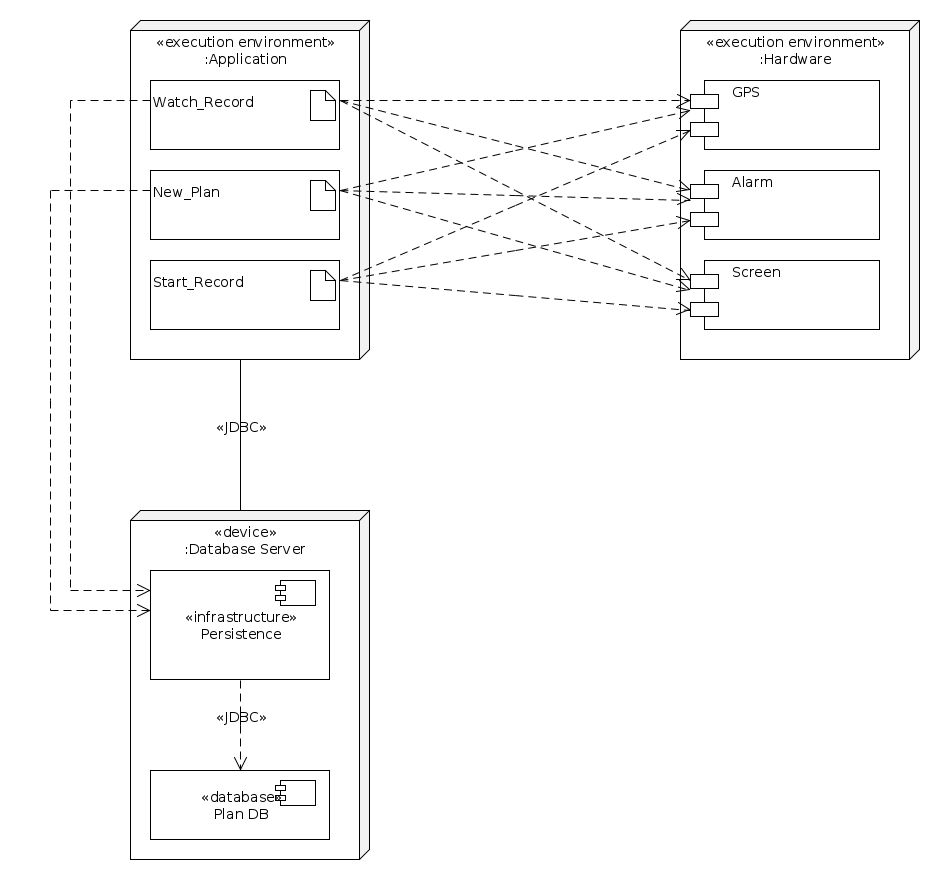
\includegraphics[width=0.75\textwidth]{SD}
			\caption{Deployment Diagram}
			\label{mylabel1}
		\end{figure}
		
\section*{实体关系模型}

\begin{figure}[ht!]
			\centering
			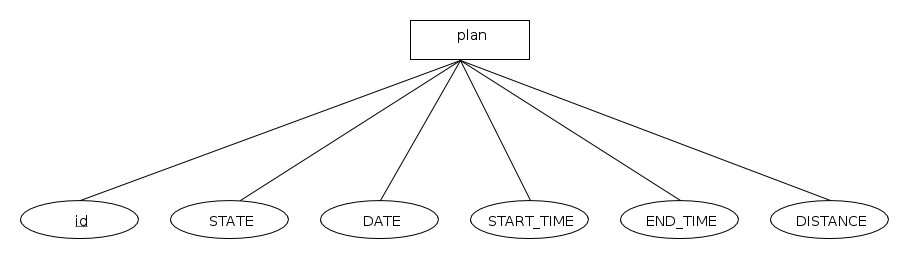
\includegraphics[width=0.9\textwidth]{ER}
			\caption{Entry Relationship model}
			\label{mylabel1}
		\end{figure}

  
\end{document}
